\documentclass{article}
\usepackage{amsmath, array, tikz, enumerate, sfmath, bm, multicol, tcolorbox}
\renewcommand{\familydefault}{\sfdefault}
\usepackage[top = 0.5in, bottom = 0.5in, left = 1in, right = 1in]{geometry}
\pagestyle{empty}
\raggedright
\tikzset{>=stealth}
\usetikzlibrary{calc}
\begin{document}

\newcounter{example}[section]
\newenvironment{example}[1][]{\refstepcounter{example}\par\medskip
   {\color{red}\textbf{Example~\theexample. #1}}}{\medskip}


\section*{Matrix Multiplication}

\begin{tcolorbox}[colframe=orange!70!white, coltitle=black, colback = white, title=\textbf{Summary}]
\begin{enumerate}
    \item Matrix multiplication creates new basis vectors $\hat{\imath}$ and $\hat{\jmath}$.
    \item An $m \times n$ matrix can be multiplied by an $n \times r$ matrix to make an $m \times r$ matrix.
    \item Matrix multiplication transforms the coordinate plane itself as a series of compositions of functions.
\end{enumerate}
\end{tcolorbox}

\subsection*{Matrix Times a Vector}

Matrix multiplication does not work the way you might think. For instance, if 
\[ 
A = 
\begin{bmatrix} 
    1 & -2 \\ 
    1 & 0 
\end{bmatrix} \quad \text{and} \quad 
B = 
\begin{bmatrix} 
    -1 & 1 \\ 
    2 & 3 
\end{bmatrix}
\]
\bigskip 

Then $AB$ is not 
$\begin{bmatrix} 
    -1 & -2 \\ 
    2 & 0 
\end{bmatrix}$. 
\bigskip

In other words, we don't multiply corresponding elements.	\bigskip 

\fbox{\fbox{
\parbox{6in}{
In order to even multiply a matrix or a vector by a vector or another matrix, {\color{blue}\textbf{the number of columns in the first matrix \emph{must} equal the number of rows in the second.}}
}
}}	
\bigskip 

Multiplying by $
\begin{bmatrix}
    1 & -2 \\ 
    1 & 0 
\end{bmatrix}$
sends $\hat{\imath}$ to 
$\begin{bmatrix} 
    1 \\ 1 
\end{bmatrix}$
and $\hat{\jmath}$ to 
$\begin{bmatrix}
    -2 \\ 0
\end{bmatrix}$
\bigskip 

\begin{center}
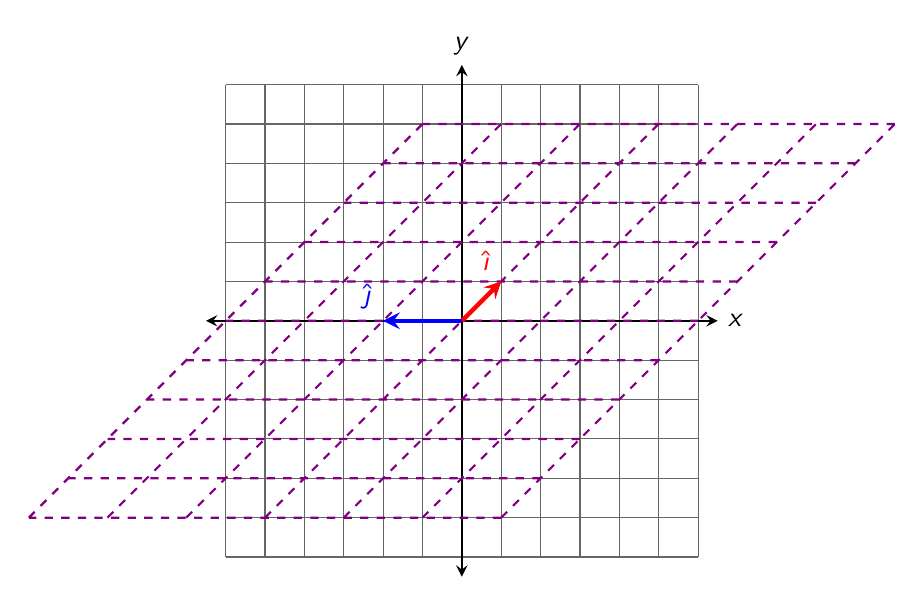
\begin{tikzpicture}[scale=0.5]
\draw[gray!120] (-6,-6) grid (6,6);
\draw[<->, thick] (-6.5,0) -- (6.5,0) node [right] {$x$};
\draw[<->, thick] (0,-6.5) -- (0,6.5) node [above] {$y$};
\pgftransformcm{1}{1}{-2}{0}{\pgfpoint{0cm}{0cm}}
\draw[violet, thick, dashed] (-5,-3) grid (5,3);
\draw[->, ultra thick, red] (0,0) -- (1,0) node [above left] {$\hat{\imath}$};
\draw[->, ultra thick, blue] (0,0) -- (0,1) node [above left] {$\hat{\jmath}$};
\end{tikzpicture}
\end{center}
\bigskip 

Notice we get a new coordinate plane (in purple). \newline\\

Along the purple coordinate plane, {\color{red}$\hat\imath$} now points along the new ``positive $x$-axis." 
\newline\\

And {\color{blue}$\hat\jmath$} now points along the new ``positive $y$-axis."
\bigskip 

\begin{center}
\fbox{\fbox{
\parbox{5in}{
Multiplying by a matrix transforms $\hat\imath$ to the first column and $\hat\jmath$ to the second column.
}}}
\end{center}

\newpage 

The following creates a new vector along our new coordinate plane (in purple):
\[
\begin{bmatrix}
    1 & -2 \\
    1 & 0 
\end{bmatrix}
\begin{bmatrix}
    1 \\ 3
\end{bmatrix}
\]

\begin{center}
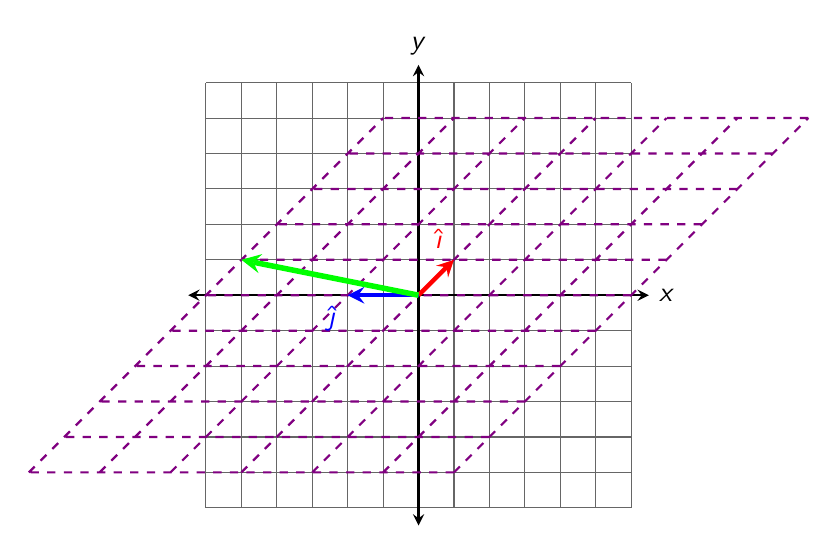
\begin{tikzpicture}[scale=0.45]
\draw[gray!120] (-6,-6) grid (6,6);
\draw[<->, thick] (-6.5,0) -- (6.5,0) node [right] {$x$};
\draw[<->, thick] (0,-6.5) -- (0,6.5) node [above] {$y$};
\pgftransformcm{1}{1}{-2}{0}{\pgfpoint{0cm}{0cm}}
\draw[violet, thick, dashed] (-5,-3) grid (5,3);
\draw[->, ultra thick, red] (0,0) -- (1,0) node [above left] {$\hat{\imath}$};
\draw[->, ultra thick, blue] (0,0) -- (0,1) node [below left] {$\hat{\jmath}$};
\draw[->, green, line width = 2] (0,0) -- (1,3);
\end{tikzpicture}
\end{center}

\begin{align*}
    \begin{bmatrix}
        1 & -2 \\ 
        1 & 0 
    \end{bmatrix}
    \begin{bmatrix}
        1 \\ 3
    \end{bmatrix}
    &= 
    1 \begin{bmatrix}
        1 \\ 1
    \end{bmatrix}
    +3 \begin{bmatrix}
        -2 \\ 0
    \end{bmatrix}   \\[10pt]
    &= \begin{bmatrix}
        1 \\ 1
    \end{bmatrix}
    + \begin{bmatrix}
        -6 \\ 0
    \end{bmatrix}   \\[10pt]
    &= \begin{bmatrix}
        -5 \\ 1
    \end{bmatrix}
\end{align*}
\vspace{0.25in}

\begin{example}
Multiply each.
\begin{enumerate}[(a)]
\begin{multicols}{2}
    \item $\begin{bmatrix}
        3 & 1 \\
        -2 & 2
    \end{bmatrix}
    \begin{bmatrix} 2 \\ -1 \end{bmatrix}$
    
    \item $\begin{bmatrix}
        -5 & -2 \\
        4 & 1 
    \end{bmatrix}
\begin{bmatrix}
        3 \\ 4
\end{bmatrix}$
\end{multicols}
\end{enumerate}
\end{example}

\vfill 
\newpage 

\subsection*{Matrix Times a Matrix}

Multiplying matrices combines matrix-vector multiplication with composition of functions; in which we evaluate the composition from the ``inside" to the ``outside" (or from right-to-left). \newline\\

For instance, in the product
\[
\begin{bmatrix} 2 & 1 \\ 1 & 2 \end{bmatrix} \begin{bmatrix}
1 & -1 \\ 1 & 3
\end{bmatrix}
\]
\bigskip 

We first look at the matrix $\begin{bmatrix} 1 & -1 \\ 1 & 3 \end{bmatrix}$ which sends $\hat{\imath}$ to $\begin{bmatrix} 1 \\ 1 \end{bmatrix}$ and $\hat{\jmath}$ to $\begin{bmatrix}
-1 \\ 3
\end{bmatrix}$. \vspace{0.25in}

\begin{center}
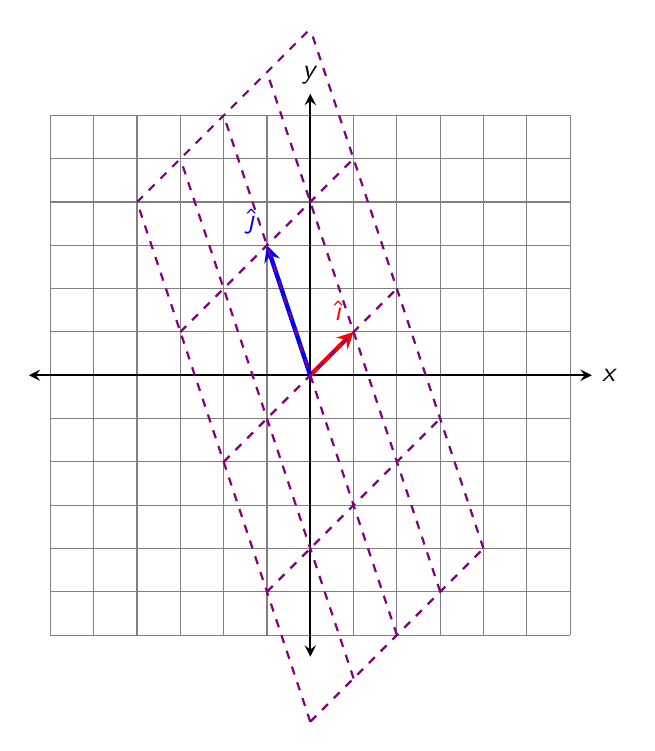
\begin{tikzpicture}[scale=0.55]
\draw[gray] (-6,-6) grid (6,6);
\draw[<->, thick] (-6.5,0) -- (6.5,0) node [right] {$x$};
\draw[<->, thick] (0,-6.5) -- (0,6.5) node [above] {$y$};
\pgftransformcm{1}{1}{-1}{3}{\pgfpoint{0cm}{0cm}}
\draw[->, ultra thick, red] (0,0) -- (1,0) node [above left] {$\hat{\imath}$};
\draw[->, ultra thick, blue] (0,0) -- (0,1) node [above left] {$\hat{\jmath}$};
\draw[violet, thick, dashed] (-2,-2) grid (2,2);
\end{tikzpicture}
\end{center}

We can then use matrix-vector multiplication to find where $\hat\imath$ and $\hat\jmath$ will end up:
\[
\begin{bmatrix} 2 & 1 \\ 1 & 2 \end{bmatrix} \begin{bmatrix}
1 & -1 \\ 1 & 3
\end{bmatrix}
\]
\begin{center}
\begin{minipage}{0.25\textwidth}
\begin{align*}
\text{Where }\hat\imath \text{ ends up} \\
\begin{bmatrix} 2 & 1 \\ 1 & 2 \end{bmatrix} 
\begin{bmatrix}
1  \\ 1 
\end{bmatrix}
% 1\begin{bmatrix}
%     2  \\
%     1  
% \end{bmatrix}
% +1\begin{bmatrix}
%     1 \\
%     2 
% \end{bmatrix}
% \\
% \begin{bmatrix}
%     2 \\ 1
% \end{bmatrix}
% +
% \begin{bmatrix}
%     1 \\ 2
% \end{bmatrix}
% \\
% \begin{bmatrix}
%     3 \\ 3
% \end{bmatrix}
\end{align*}
\end{minipage}
%%%%
\begin{minipage}{0.35\textwidth}
\begin{align*}
\text{Where }\hat\jmath \text{ ends up} \\
\begin{bmatrix} 2 & 1 \\ 1 & 2 \end{bmatrix} 
\begin{bmatrix}
-1 \\ 3 
\end{bmatrix}
% \\
% -1\begin{bmatrix}
%     2  \\
%     1  
% \end{bmatrix}
% +3\begin{bmatrix}
%     1 \\
%     2 
% \end{bmatrix}
% \\
% \begin{bmatrix}
%     -2 \\ -1
% \end{bmatrix}
% +
% \begin{bmatrix}
%     3 \\ 6
% \end{bmatrix}
% \\
% \begin{bmatrix}
%     1 \\ 5
% \end{bmatrix}
\end{align*}
\end{minipage}
\end{center}
\vfill 
% \[
% \begin{bmatrix} 2 & 1 \\ 1 & 2 \end{bmatrix} \begin{bmatrix}
% 1 & -1 \\ 1 & 3
% \end{bmatrix} = 
% \begin{bmatrix}
%     3 & 1 \\
%     3 & 5 
% \end{bmatrix}
% \]

\newpage

\begin{example}
Multiply each of the following.
\begin{enumerate}[(a)]
\begin{multicols}{2}
    \item 
    $\begin{bmatrix} 
        0 & -1 \\
        1 & 0 
    \end{bmatrix} 
    \begin{bmatrix}
        1 & 2 \\
        0 & 1 
    \end{bmatrix}$
    
    \item 
    $\begin{bmatrix}
        1 & 2 \\
        0 & 1
    \end{bmatrix}
    \begin{bmatrix} 
        0 & -1 \\
        1 & 0 
    \end{bmatrix}$
\end{multicols}
\vspace{5in}
    
    \item Does the order in which we multiply matrices matter?
    \vspace{1in} 
\end{enumerate}
\end{example}

\newpage 

\subsection*{When Matrix Multiplication May Fail}

Sometimes we run out of components when multiplying a matrix times a vector. \newline\\

\emph{This will happen if the number of columns in the first matrix do not equal the number of rows in the second matrix.}    
\bigskip 

Otherwise, we will end up with a matrix where 
\begin{align*}
    \text{number of rows} &= \text{number of rows of 1st matrix} \\
    \text{number of columns} &= \text{number of columns of 2nd matrix}
\end{align*}
\bigskip 

\begin{example} 
Multiply each (if possible).
\end{example}
\begin{enumerate}[(a)]
    \item 
    $\begin{bmatrix}
        2 & 4 \\ -2 & 3 \\ 5 & 1
    \end{bmatrix}
    \begin{bmatrix}
        -3 & 6 \\ 0 & -2 
    \end{bmatrix}$
    \newpage  
    
    \item 
    $\begin{bmatrix}
        -3 & 6 \\ 0 & -2 
    \end{bmatrix}
    \begin{bmatrix} 
        2 & 4 \\ -2 & 3 \\ 5 & 1
    \end{bmatrix}$
    \vfill  
    
    \item 
    $\begin{bmatrix}
        4 & -1 \\ 5 & 1 
    \end{bmatrix}
    \begin{bmatrix}
        2 & 3 & -1 \\ 0 & 1 & 4
    \end{bmatrix}$
    \vfill 
    % \newpage
    
    % \item
    % $\begin{bmatrix}
    %     0 & 2 & -1 \\ 4 & 1 & 0 \\ 0 & -1 & 2
    % \end{bmatrix}
    % \begin{bmatrix}
    %     4 & 3 & 0 \\ -1 & 0 & 2 \\ 1 & 0 & -2
    % \end{bmatrix}$
    % \vfill 
\end{enumerate}




 
 
\end{document}